% include the figures path relative to the master file
\graphicspath{ {./content/method/figures/} }
\section{Review}\label{sec:review}
This section reviews the recent and the state-of-the-art methods in
classification of \gls{sdoct} volumes as normal vs. abnormal.  These methods
can be categorized into two groups, supervised and semi-supervised explained in
the following.

% Common framework
\added[id=mojh]{ All the previously mentioned methods follow a similar pipeline
  or framework, which consists of different steps.  We categorized these steps
  as pre-processing, feature extraction, mapping, feature representation and
  finally classification, as it is shown in Fig.\,\ref{fig:ML-scheme}.
  Pre-processing of \gls{oct} volumes, as noted in Sect.\,\ref{sec:review},
  consists of denoising, flattening the retinal curvature, aligning the B-scans
  through the whole volume and finally cropping or resizing the volumes.
  Feature extraction refers to extraction of different textural and shape
  information from the B-scan or the volumes.  Mapping step is used to
  determine a discrete set of elements (structures) representing a sample (i.e.
  B-scan/volume).  In this step either one structure is used per sample namely
  global-mapping or the features are extracted with reference to a set of
  structures, i.e. dense or sparse patches through the sample, local-mapping.
  In feature representation step, the representation of the final descriptor
  prior to classification is decided.  The extracted features using different
mapping techniques can be represented in lower dimensions (using \gls{pca} for
instance), as a concatenated of descriptor, histogram of words (using
\gls{bow}) or sparse representation (sparse coding).}

Supervised classification is based on full annotated and labeled training set.
In such methods the labeled training data is used to train the classifier
function and the learned function is used for prediction.  Semi-supervised
classification takes advantage of both unlabeled and labeled data.  This
techniques are particularly useful when there is lack of annotated data
moreover it has shown that use of small amount of labeled data in conjunction
of unlabeled data can increase the learning accuracy.

The details implementation of the following methods and their integration to
our common framework is described in Sect.~\textit{experiments}.
%\added[id=old]{ This section reviews the works straightly addressing the
%problem of classifying \gls{oct} volumes as normal or abnormal.}
%Implementation details in order to integrate all these methodologies in
%a common framework can be found in Sect.\,\ref{sec:method} and further details
%in all the repositories
%available~\cite{repo_srini,repo_ven,repo_liu,repo_des,repo_lem}.
\subsection{Supervised methods}

Venhuizen \textit{et al.} proposed a supervised method for \gls{sdoct} image
classification using \gls{bow} models~\cite{Venhuizen2015}.  With the aim of
\gls{amd} versus normal volumes classification, the method starts with the
detection and selection of keypoints in each individual B-scan. %by keeping the
most salient points corresponding to the top $3 \%$ of the vertical gradient
values.  The final keypoints are selected as the most salient points
corresponding to the top $3 \%$ of the vertical gradient values.  Then,
a texton of size $9 \times 9$ pixels is extracted around each keypoint, and
\gls{pca} is applied to reduce the dimension of every texton to get a feature
vector of size $9$.  All extracted feature vectors are used to create
a codebook using \textit{k}-means clustering.  Then, each volume is represented
in terms of created codebook and is characterized as a histogram that captures
the codebook occurrences.  These histograms are used as feature vector to train
a \gls{rf} with a maximum of $100$ trees.  Using the proposed method the
authors achieved an \gls{auc} of $0.984$ with a dataset of $384$ volumes.
%The method was used to classify \gls{oct} volumes between \gls{amd} and normal
%cases and achieved an \gls{auc} of $0.984$ with a dataset of $384$ \gls{oct}
%volumes.

Another supervised method is proposed by Srinivasan
\textit{et~al.}~\cite{Srinivasan2014} which intends to distinguish \gls{dme},
\gls{amd} and normal \gls{sdoct} volumes.
%Srinivasan\,\textit{et~al.}~\cite{Srinivasan2014} proposed a classification
%method to distinguish \gls{dme}, \gls{amd} and normal \gls{sdoct} volumes.
In this method in order to reduce the inter-patient variations, the \gls{oct}
images are pre-processed by first enhancing sparsity in a transform-domain
(BM3D~\cite{dabov2007image}), to reduce their speckle noise, and then by
flattening the retinal curvature.  The denoised and flatten B-scans are further
cropped to reduce the size and therefore complexity of the algorithm.
%The \gls{oct} images are pre-processed by reducing the speckle noise by
%enhancing the sparsity in a transform-domain and flattening the retinal
%curvature to reduce the inter-patient variations.
The \gls{hog} features are then extracted from multi-resolution pyramid of each
pre-processed slice of a volume.  These features are classified using a linear
\gls{svm}.  Note that the method classifies each individual B-scan into one of
three categories, i.e. \gls{dme}, \gls{amd}, and normal, and then classifies
a volume based on the number of B-scans in each category.
%Then, \gls{hog} are extracted for each slice of a volume and a linear
%\gls{svm} is used for classification.
On a balanced dataset of 45 patients, this method leads to correct
classification rate of $100 \%$, $100 \%$ and $86.67 \%$ for normal, \gls{dme}
and \gls{amd} patients, respectively.
%On a dataset of 45 patients equally subdivided into the three aforementioned
%classes, this method leads to a correct classification rate of $100 \%$, $100
%\%$ and $86.67 \%$ for normal, \gls{dme} and \gls{amd} patients, respectively.

%The images that have been used in their paper, are publicly available but are
%already preprocessed (i.e., denoised), have different sizes for the \gls{oct}
%volumes, do not offer a huge variability in term of \gls{dme} lesions, and
%some of them, without specifying which, have been excluded for the training
%phase; all these reasons prevent us from using this dataset to benchmark our
%work.

Replicating the method proposed by Srinivasan
\textit{et~al.}~\cite{Srinivasan2014} and adding \gls{pca} to the feature
extraction step, as was proposed by Venhuizen \textit{et
al.}~\cite{Venhuizen2015}, we also compare the performance of extracted
\gls{hog} and \gls{lbp} features (similar to \cite{Srinivasan2014}, features
are extracted from multi-resolution pyramid) for classification of B-scans, and
accordingly volumes.  {\color{red}This work was submitted for publication to
a recent conference.}

Lemaitre \textit{at~al.}~\cite{Lemaintre2015miccaiOCT} proposed another method
based on extracted \gls{lbp} features from \gls{oct} images and dictionary
learning using \gls{bow} models~\cite{Sivic2003}.
%The proposed method by Lemaitre~\emph{et~al.}~\cite{Lemaintre2015miccaiOCT} is
%based on \gls{lbp} features to describe the texture of \gls{oct} images and
%dictionary learning using the \gls{bow} models~\cite{Sivic2003}.
Note that using \gls{bow} and dictionary learning contrary to
\cite{Srinivasan2014} the classification is performed per volume, rather than
B-scan.  In this method the \gls{oct} images are first pre-processed using
\gls{nlm} filtering, to reduce the speckle noise.
%The data is pre-processed using \gls{nlm} filtering.
Then the volumes are mapped into discrete set of structures namely: local, when
these structures correspond to patches; or global, when they correspond to
volume slices or the whole volume.  According to different mapping, \gls{lbp}
or \gls{lbptop} texture features are extracted and represented (per volume)
using histogram, \gls{pca} or \gls{bow}.  The final feature descriptors per
volumes are classified using \gls{rf} classifier.  Classifying \gls{dme} versus
normal volumes with a balanced dataset of 32 \gls{sdoct} volumes, they achieved
a \gls{se} and \gls{sp} of 87.50\% and 75\%, respectively, while using
\gls{lbptop} features and global mapping.
%These structures are described in terms of texture using \gls{lbp} or
%\gls{lbptop} and encoded using histogram, \gls{pca} or \gls{bow} to produce
%a single feature vector in order to present the volumes to a \gls{rf}
%classifeir.  This methodology was tested against Venhuizen\,\textit{et
%al.}~\cite{Venhuizen2015} using public and non-public datasets showing an
%improvement within the results achieving a \gls{se} of 87.5\% and a \gls{sp}
%of 75\%.  Our later study proposes a standard classification procedure to
%differentiate between \gls{dme} and normal \gls{sdoct}
%volumes~\cite{Lemaitre2015}

Another supervised method is proposed by Liu \textit{et al.}~\cite{Liu2011},
with the specific aim of B-scan classification, rather than volume
classification.  In this study, the authors proposed to extract \gls{lbp} and
gradient information (using \gls{lbp} on canny-edged B-scans) from
pre-processed \gls{oct} images.  The pre-processing is performed by flattening
and aligning \gls{oct} images in a volume.  The features are then extracted
from spatial blocks of $3$-level multi-scale spatial pyramid of each B-scan.
All the obtained histograms are concatenated into a global descriptor whose
dimensions are reduced using \gls{pca}.  Finally a \gls{svm} with an \gls{rbf}
kernel is used as classifier.  The method achieved good results in detection of
\gls{oct} scans containing different pathology such as \gls{dme} or \gls{amd},
with an \gls{auc} of $0.93$ using a dataset of $326$ \gls{oct} scans.


%Liu\,\textit{et al.} proposed a methodology for detecting macular pathology in
%\gls{oct} images using \gls{lbp} and gradient information as
%attributes~\cite{Liu2011}.  The method starts by aligning and flattening the
%images and creating a $3$-level multi-scale spatial pyramid.  The edge and
%\gls{lbp} histograms are then extracted from each block of every level of the
%pyramid.  %is created and edge and \gls{lbp} histograms are extracted in each
%block at every level of the pyramid.  All the obtained histograms are
%concatenated into a global descriptor whose dimensions are reduced using
%\gls{pca}.  Finally a \gls{svm} with an \gls{rbf} kernel is used as
%classifier.  The method achieved good results in detection \gls{oct} scan
%containing different pathology such as \gls{dme} or \gls{amd}, with an
%\gls{auc} of $0.93$ using a dataset of $326$ \gls{oct} scans.



\subsection{Semi-supervised methods}
An example of semi-supervised approach for \gls{sdoct} classification is
recently proposed by Sankar. \textit{et al.}~\cite{sankar2016classification}.
The proposed method is based on appearance modeling of normal \gls{oct} images
using \gls{gmm} and anomaly detection.  The abnormal B-scans are detected as
outliers to the fitted \gls{gmm} and volume classification is performed based
on the number of detected outliers in the volume.

%The proposed method is based on modeling the appearance of the normal
%\gls{oct} images using a \gls{gmm} and detecting abnormal \gls{oct} images as
%outliers.  Use an anomaly detection approach to identify abnormal B-scan as
%outliers to the \gls{gmm} and finally detect unhealthy \gls{oct} volumes based
%on the number of abnormal B-scan.
This approach differs from supervised approaches since the B-scan detection
method does not require a labeled training set of B-scans.  This method starts
by pre-processing the B-scans using resizing, flattening and denoising
(\gls{nlm} filter).  The features are extracted by taking the intensity
information of each B-scan and applying \gls{pca} to reduce their dimension.
The feature space is then modeled using \gls{gmm}.  In the testing stage, for
the new B-scan, the features are extracted in a similar way and they are
classified as normal or abnormal based on their Mahalanobis distance to the
\gls{gmm}.  Finally the volume classification is performed considering the
umber of outliers (abnormal) B-scans per volume.


Table~\ref{tab:survey-tab} summarizes the aforementioned methods in terms of
the proposed framework.

\begin{figure*}
  \centering{
  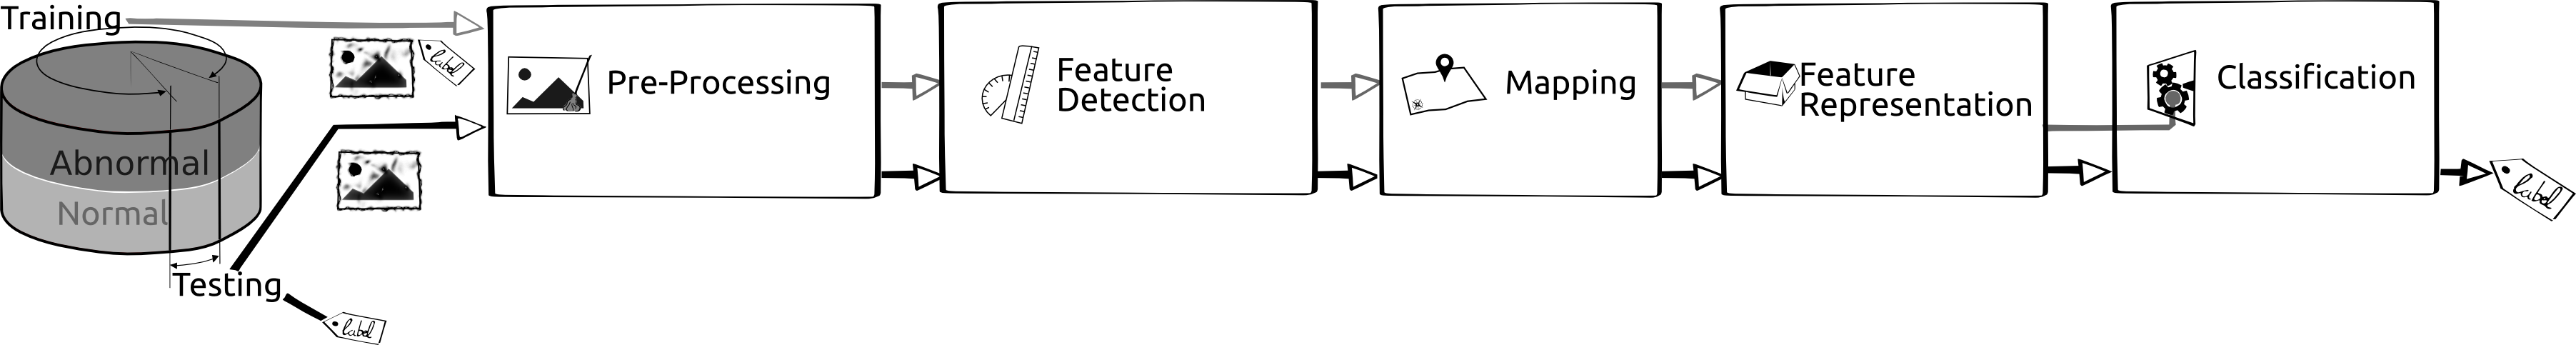
\includegraphics[width=1\linewidth]{ml-2}}
  \caption{Common framework}
  \label{fig:ML-scheme}
\end{figure*}

\begin{table}
  \caption{Correspondence between the most relevant methodologies reviewed in Sect.\,\ref{sec:review} and the proposed experimental framework.}
\resizebox{1\linewidth}{!}{
\footnotesize{
\begin{tabular}{l c	c c c c }
\toprule
\multicolumn{1}{c}{Ref} & Pre-processing & Features &  Mapping &  Representation & Classification\\
    &  &  &  &  & \\
\midrule
	&  &  &  &  & \\
%Venhuizen\,\textit{et al.}~
Venhuizen \textit{et al.}~\cite{Venhuizen2015,venhuizen2015feb-repoICPR} &  & Texton & Local   &\gls{bow}, \gls{pca}  & \gls{rf} \\
	&  &  &  &  & \\
%Srinivansan\,\textit{et al.}~
\multirow{3}{*}{Srinivasan \textit{et al.}~\cite{Srinivasan2014, srinivasan2014oct-repoICPR}} & De-noise & \multirow{3}{*}{\gls{hog}} & \multirow{3}{*}{Global} & &  \multirow{3}{*}{linear-\gls{svm}} \\
 & Flatten & & & & \\
 & Cropped & & & & \\
	&  &  &  &  & \\
%Lema\^itre\,\textit{et al.}~
Lemaitre \textit{et al.}~\cite{Lemaintre2015miccaiOCT, lemaitre2015apr-repoICPR} & De-noised & \gls{lbp} & Local &  \gls{pca}, &  \gls{rf} \\
& & \gls{lbptop} & Global & \gls{bow}, Histogram & \\ 
	&  &  &  &  & \\

Alsaih \textit{et al.}~\cite{Alsaih2016apr-repoICPR} & ********* & \gls{lbp} & ***** &  \gls{pca}, &  \gls{rf} \\
& & \gls{lbptop} & ****** & \gls{bow}, ********* & \\ 
	&  &  &  &  & \\

%Liu\,\textit{et al.}~
% \multirow{2}{*}{Liu \textit{et al.}~\cite{Liu2011}} & Flatten & \multirow{2}{*}{Edge, \gls{lbp}} & \multirow{2}{*}{Local} & \multirow{2}{*}{\gls{pca}}& \multirow{2}{*}{\gls{rbf}-\gls{svm}} \\
% & Aligned & & & & \\
% 	&  &  &  &  & \\

%\midrule
\hdashline \noalign{\vskip 3pt}
\multirow{3}{*}{Sankar \textit{et al.}~\cite{sankar2016classification, sankar2015feb-repoICPR}} & De-noised & Pixel & \multirow{3}{*}{Global} & \multirow{3}{*	}{\gls{pca}} & Mahalanobis \\
 & Flatten &-intensities & & & -distance\\
 & Cropped & & & & to \gls{gmm}\\ 
\bottomrule
\end{tabular}}
}
\label{tab:survey-tab}
\end{table}

%\begin{table*}
%\caption{Summary of the state-of-the-art methods.}
%\resizebox{1.05\linewidth}{!}{
%\scriptsize{
%\begin{tabular}{l ccc c cccc	c c c c	c c}
%\toprule
%Ref & \multicolumn{3}{c}{Diseases} & Data  & \multicolumn{4}{c}{Pre-processing} & Features & Representation & Classifier & Evaluation & Results\\
%    &  &  &  & size &  &  &  &  &  &  &  & & &\\
%   \cmidrule(l){2-4}\cmidrule(l){6-9} 
%    & \gls{amd} & \gls{dme} & Normal  &           & De-noise & Flatten & Aligning & Cropping &   & &   &  &   \\
%\midrule
%& & & & & & & & & & & & & &  \\
%%Srinivansan\,\textit{et al.}~
%\cite{Srinivasan2014} & $\checkmark$ & $\checkmark$ & $\checkmark$ &  45 & $\checkmark$ & $\checkmark$ &  & $\checkmark$ & \gls{hog} &  & linear-\gls{svm} & \gls{acc} & 86.7\%,100\%,100\%  \\
%& & & & & & & & & & & & &    \\
%%Venhuizen\,\textit{et al.}~
%\cite{Venhuizen2015} & $\checkmark$ &  & $\checkmark$ & 384 &  & & & &  Texton  &\gls{bow}, \gls{pca}  & \gls{rf} & \gls{auc} & 0.984 \\ 
%& & & & & & & & & & & & &   & \\
%%Liu\,\textit{et al.}~
%\cite{Liu2011} & $\checkmark$ & $\checkmark$ & $\checkmark$  & 326 &  & $\checkmark$ & $\checkmark$ &  &  Edge, \gls{lbp} & \gls{pca}& \gls{svm}-\gls{rbf} &\gls{auc} & 0.93 \\
%& & & & & & & & & & & & & \\
%%Lema\^itre\,\textit{et al.}~
%\cite{Lemaintre2015miccaiOCT} &  & $\checkmark$ & $\checkmark$ & 62  & $\checkmark$ &  &  &  & \gls{lbp}-\gls{lbptop} & \gls{pca}, \gls{bow}, histogram&  \gls{rf} & \gls{se},\gls{sp} & 87.5\%, 75\%  \\
%& & & & & & & & & & & & &  \\
%\bottomrule
%\end{tabular}}}
%\label{tab:survey-tab}
%\end{table*}



\section{\replaced[id=sik]{Experimental Setup}{Materials and Methods}}
\label{sec:method}\label{sec:exp}

%The experimental set-up is formulated as a standard classification procedure
%consisting of 5 steps.  Figure~\ref{fig:ML-scheme} outlines these 5 steps and
%illustrates how the methodologies have been translated to such schema.

%\begin{figure*} \centering{ 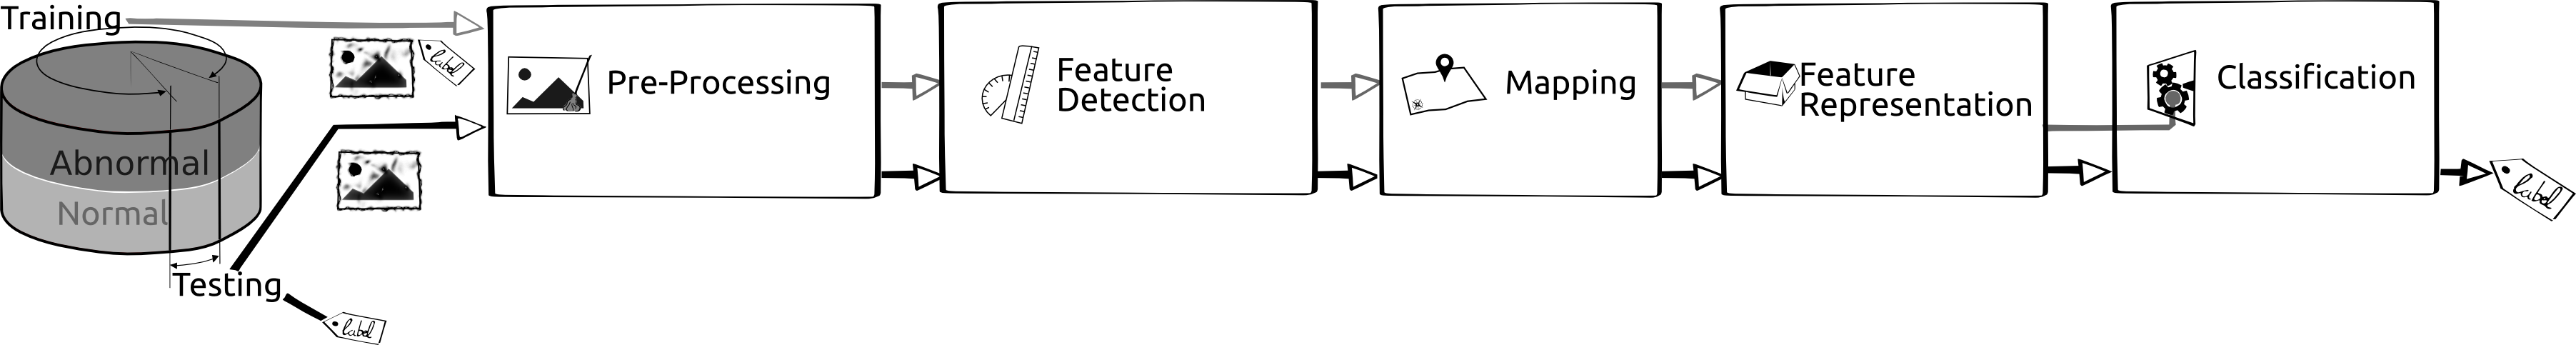
\includegraphics[width=1\linewidth]{ml-2}}
%  \caption{Experimental Setup} \label{fig:ML-scheme} \end{figure*}


\subsection{\deleted[id=sik]{method comments}}
\todo[inline]{
  here goes a description left to right of the modules, making remarks of the
  difference between the needs of each method.
}
\added[id=old]{
  First, the \gls{oct} volumes are pre-processed as presented in details in
  Sect.\,\ref{subsec:prepro}.
%Then toward a final descriptor \gls{lbp} and \gls{lbptop} features are
  %extracted with different mapping strategy and represented using two
  %approach.
Then, \gls{lbp} and \gls{lbptop} features are detected, mapped and represented
as discussed in depth in Sect.\,\ref{subsec:feaext},
Sect.\,\ref{subsec:mapping}, and Sect.\,\ref{subsec:fearep}, respectively.
%{\color{red}The feature extraction, mapping, and representation are presented
%in depth in Sect.\,\ref{subsec:feaext}, Sect.\,\ref{subsec:mapping}, and
%Sect.\,\ref{subsec:fearep}, respectively. CHECK THE SECTION ORDERING}
Finally, the classification step is presented in Sect.\,\ref{subsec:cls}.
}

